
\documentclass[UTF8,AutoFakeBold,AutoFakeSlant,zihao=-4]{ctexart}
\usepackage[a4paper,left=2.4cm,right=2.4cm,top=2.6cm,bottom=2.38cm,includeheadfoot]{geometry}
\usepackage{fontspec}
\usepackage{setspace}
\usepackage{graphicx}
\usepackage{fancyhdr}
\usepackage{pdfpages}
\usepackage{setspace}
\usepackage{booktabs}
\usepackage{multirow}
\usepackage{caption}

% 设置参考文献编译后端为 biber,引用格式为 GB/T7714-2015 格式
% 参考文献使用宏包见 https://github.com/hushidong/biblatex-gb7714-2015
\usepackage[style=gb7714-2015,backend=biber]{biblatex}

% 参考文献引用文件 refs.bib
\addbibresource{misc/refs.bib}

\newcommand{\coursename}{《Python程序设计》}
\newcommand{\coursenumber}{U08M11077.01}
\newcommand{\proname}{2048小游戏开发}
\newcommand{\members}{敖冠舒~唐中磊~王骏松~王一帆}
\newcommand{\phone}{134~0324~7575}
\newcommand{\protime}{2022年12月}

% 定义 caption 字体为楷体
\DeclareCaptionFont{kaiticaption}{\kaishu \normalsize}

% 设置图片的 caption 格式
\renewcommand{\thefigure}{\thesection-\arabic{figure}}
\captionsetup[figure]{font=small,labelsep=space,skip=10bp,labelfont=bf,font=kaiticaption}

% 设置表格的 caption 格式
\renewcommand{\thetable}{\thesection-\arabic{table}}
\captionsetup[table]{font=small,labelsep=space,skip=10bp,labelfont=bf,font=kaiticaption}

% 定义一个概念
\newtheorem{definition}{概念}[section]

% 输出大写数字日期
\CTEXoptions[today=big]


\setromanfont{Times New Roman}

%% 将中文楷体设置为 SIMKAI.TTF(如果需要)
% \setCJKfamilyfont{zhkai}{[SIMKAI.TTF]}
% \newcommand*{\kaiti}{\CJKfamily{zhkai}}

% 设置文档标题深度
\setcounter{tocdepth}{3}
\setcounter{secnumdepth}{3}

%%
% 设置一级标题、二级标题格式
% 一级标题:小三,宋体,加粗,段前段后各半行
\ctexset{section={
  format={\raggedright \bfseries \songti \zihao{-3}},
  beforeskip = 24bp plus 1ex minus .2ex,
  afterskip = 24bp plus .2ex,
  fixskip = true,
  name = {,.\quad}
  }
}
% 二级标题:小四,宋体,加粗,段前段后各半行
\ctexset{subsection={
  format = {\bfseries \songti \raggedright \zihao{4}},
  beforeskip =24bp plus 1ex minus .2ex,
  afterskip = 24bp plus .2ex,
  fixskip = true,
  }
}

%%
% 文档开始
\begin{document}

% 报告封面
\topskip=0pt

\begin{titlepage}
  \vspace*{20mm}
  \centering
  \hspace{0mm}\heiti\fontsize{30pt}{30pt}\selectfont{西北工业大学}

  \vspace{13mm}

  \hspace{0mm}\heiti\fontsize{20pt}{20pt}\selectfont{课程设计(大作业)报告}

  \vspace{40mm}

  \flushleft
  \begin{spacing}{2.2}


    \hspace{36mm}\songti\fontsize{16pt}{16pt}\selectfont{\textbf{课程名称:}\underline{\makebox[72mm][c]{\coursename}}}

    \hspace{36mm}\songti\fontsize{16pt}{16pt}\selectfont{\textbf{课程编号:}\underline{\makebox[72mm][c]{\coursenumber}}}

    \hspace{36mm}\songti\fontsize{16pt}{16pt}\selectfont{\textbf{设计题目:}\underline{\makebox[72mm][c]{\proname}}}

    \hspace{36mm}\songti\fontsize{16pt}{16pt}\selectfont{\textbf{组员名单:}\underline{\makebox[72mm][c]{\members}}}

    \hspace{36mm}\songti\fontsize{16pt}{16pt}\selectfont{\textbf{联系方式:}\underline{\makebox[72mm][c]{\phone}}}

    \hspace{36mm}\songti\fontsize{16pt}{16pt}\selectfont{\textbf{设计时间:}\underline{\makebox[72mm][c]{\protime}}}
  \end{spacing}

  \vspace{47mm}


\end{titlepage}




%%
% 正文开始
\pagestyle{fancy}
% 正文从第一页开始计算页码
\setcounter{page}{1}
% 页眉和页脚(页码)的格式设定
\fancyhf{}
\fancyhead[R]{\fontsize{10.5pt}{10.5pt}\selectfont{西北工业大学课程设计(大作业)报告}}
\fancyfoot[R]{\fontsize{9pt}{9pt}\selectfont{\thepage}}
\renewcommand{\headrulewidth}{1pt}
\renewcommand{\footrulewidth}{0pt}

% 正文 22 磅的行距,段前段后间距为 0
\setlength{\parskip}{0em}
\renewcommand{\baselinestretch}{1.53}
% 正文首行悬挂 1.02cm
\setlength{\parindent}{1.02cm}

% 内容开始
\section{毕业设计(论文)选题的内容}
开题报告总长度约 5 至 6 页,本部分重点介绍毕业设计选题的主要内容 \cite{LeCun2010},宋体,小三,段落前后 0.5 行。

\section{研究方案}
\subsection{本选题的主要任务}
本部分重点关注毕业设计的主要任务,宋体,四号,段落前后 0.5 行。

\subsection{技术方案的分析、选择}
此部分要分析任务书,并给出初步方案,要体现出复杂系统的概念,约写 2 至 3 页。

\begin{figure}[!ht]
  \centering
  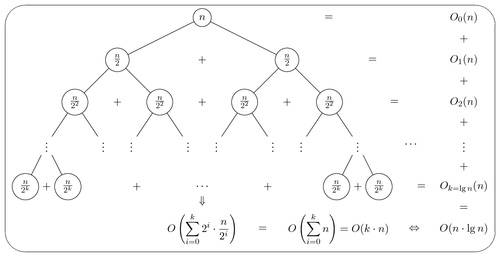
\includegraphics[width=0.6\linewidth]{merge-sort-recursion-tree}
  \caption{Merge sort recursion tree:一张示意图}
  \label{fig:mergesort}
\end{figure}

\subsubsection{第一阶段}
在第一阶段,我们准备……

\subsection{实施技术方案所需的条件}
此部分说明所需的软硬件等环境,建议使用表格的形式,方便表述。

\begin{table}[!ht]
  \centering
  \caption{硬件、软件环境}
  \label{tab:soft-hardware}
  \begin{tabular}{@{}lcl@{}}
    \toprule
                              & 指标     & \multicolumn{1}{c}{版本参数} \\ \midrule
    \multirow{2}{*}{硬件环境} & CPU      & Intel i7-6500U               \\ \cmidrule(l){2-3}
                              & RAM      & 8 GB                         \\ \midrule
    \multirow{2}{*}{软件环境} & 操作系统 & \begin{tabular}[c]{@{}l@{}}Windows 10 Pro x86\_64\\  Ubuntu 18.04.3 LTS\end{tabular}    \\ \cmidrule(l){2-3}
                              & Python   & Python 3.7.6                 \\ \bottomrule
  \end{tabular}
\end{table}

\subsection{存在的主要问题和技术关键}
目前存在的主要问题是……

正文,小四,行距 22 磅。

\subsection{预期能够达到的研究目标}
要包括最后提交的成果。

\section{课题计划进度表}
大致的课题计划进度如下表 \ref{tab:progress} 所示。

\begin{table}[!ht]
  \centering
  \caption{毕业设计计划进度表}
  \label{tab:progress}
  \begin{tabular}{@{}cllc@{}}
    \toprule
    阶段 & \multicolumn{1}{c}{任务} & \multicolumn{1}{c}{完成标志} & 时间规划       \\ \midrule
    1    & 第一阶段的任务……          & 成功搭建……                    & 2019.12-2020.1 \\ \midrule
    2    & 第二阶段的任务……          & 成功验证……                    & 2020.1-2020.2  \\ \midrule
    3    & 第三阶段的任务……          & 成功验证……失效,并优化……增强  & 2020.2-2020.4  \\ \midrule
    4    & 第四阶段的任务……          & 成功完成毕业设计              & 2020.4-2020.5  \\ \bottomrule
  \end{tabular}
\end{table}

注意:下文的参考文献应包含近 5 年内文献,经典文献除外。

\section{参考文献}
% 删除默认的「参考文献 / Reference」标题,使用上面定义的 section 标题
\printbibliography[heading=none]

\end{document}
